\section*{Introduction}
Dans le contexte, décrire le problème (de L’ADT) et à quoi ça sert.\\
Transcrire des solos, intérêt $\Rightarrow$ constitution de corpus musicologique.\\
Digression sur la musicologie calculatoire (vs linguistique computationnelle).\\
Édition de partition.\\
L’ADT a engendré une pluie de sous-tâche qui a donné naissance au MIR. 
Dans ce chapitre, nous présenterons le rapport possible entre la musique et le TAL, en considérant les notions de langage musical et langue naturelle, le lien entre partition musicale comme manière d’écrire la musique et texte comme manière d’écrire la parole.\\
Nous aborderons aussi les applications des techniques TAL pour les différents traitements associés à la musique et nous ferons un tour d’horizon des domaines de la recherche d’information musicale.\\ Nous présenterons ensuite le problème de la transcription automatique de la musique.

\section{Informatique musicale}
\cite{first_one}
\section{TAL et MIR}
Aborder la musique à travers le TAL nécessite une réflexion autour de la musique en tant que langage ainsi que la possibilité de comparer ce même langage avec les langues naturelles. Quelques travaux en neuroscience ont abordé la question, notamment par observation des processus cognitifs et neuronaux que les systèmes de traitement de ces deux langages avaient en communs. Dans le travail de Poulin-Charronnat et al. \cite{poulincharronnat:hal-01985213}, la musique est reconnue comme étant un système complexe spécifique à l’être humain dont une des similitudes avec les langues naturelles est l’émergence de régularités reconnues implicitement par le système cognitif. La question de la pertinence de l’analogie entre langues naturelles et langage musical a également été soulevée à l’occasion de projets de recherche en TAL. Keller et al. \cite{keller:hal-03279850} ont exploré le potentiel de ces techniques à travers les plongements de mots et le mécanisme d’attention pour la modélisation de données musicales. La question du sens d’une phrase musicale apparaît, selon eux, à la fois comme une limite et un défi majeur pour l’étude de cette analogie.\\
D’autre travaux très récents, ont aussi été révélé lors de la \textit{première conférence sur le NLP pour la musique et l'audio (NLP4MusA 2020)}. Lors de cette conférence, Jiang et al. \cite{Jiang2020DiscoveringMR} ont présenté leur implémentation d’un modèle de langage musical auto-attentif visant à améliorer le mécanisme d'attention par élément, déjà très largement utilisé dans les modèles de séquence modernes pour le texte et la musique.
\section{La transcription automatique de la musique}
Problème vieux et difficile $\Rightarrow$ c’est un graal.
Voir l’intro de \cite{article1}\\
L'objectif de la transcription automatique de la musique (AMT) \cite{article1} est de convertir la performance d'un musicien en notation musicale - un peu comme la conversion de la parole en texte dans le traitement du langage naturel. Bien que l’AMT soit un domaine de recherche en plein essor dans lequel plusieurs approches différentes sont encore activement étudiées, les performances des systèmes actuels ne sont pas encore suffisantes pour certaines applications qui exigent un haut degré de précision \cite{article1}. Même si les applications typiques de l'AMT comprennent l'estimation de la multi-tonalité, la classification des genres musicaux, la détection du début et de la fin des notes de musique, l'estimation du tempo, le suivi du rythme et la transcription de la musique. La plupart des travaux se sont concentrés sur le traitement du signal vers la génération du midi \cite{article2}. Seuls quelques travaux récents \cite{foscarin:hal-01988990} s’intéressent de près à la création d’outils permettant la génération de partition.
%\subsection*{Définition}
%\subsection{transcription musicale automatique}
Le terme « transcription musicale automatique » a été utilisé pour la première fois par les chercheurs en audio James A. Moorer, Martin Piszczalski et Bernard Galler en 1977. Grâce à leurs connaissances en ingénierie audio numérique, ces chercheurs pensaient qu'un ordinateur pouvait être programmé pour analyser un enregistrement numérique de musique de manière à détecter les hauteurs des lignes mélodiques et des motifs d'accords, ainsi que les accents rythmiques des instruments à percussion.\\La tâche de transcription automatique de la musique comprend deux activités distinctes : l'analyse d'un morceau de musique et l'impression d'une partition à partir de cette analyse.\footnote{\url{https://en.wikipedia.org/wiki/Transcription_(music)}}
\section{Les partitions}
Mettre une image de partition ici
Une partition de musique\footnote{\url{https://fr.wikipedia.org/wiki/Partition\_(musique)}} est un document qui porte la représentation systématique du langage musical sous forme écrite. Cette représentation est appelée transcription et elle sert à traduire les quatre caractéristiques du son musical :
\begin{itemize}
	\item la hauteur ;
	\item la durée ;
	\item l'intensité ;
	\item le timbre.
\end{itemize}
Ainsi que de leurs combinaisons appelées à former l'ossature de l'œuvre musicale dans son déroulement temporel, à la fois :
\begin{itemize}
	\item diachronique (succession des instants, ce qui constitue en musique la mélodie) ;
	\item et synchronique (simultanéité des sons, c'est-à-dire l'harmonie).
\end{itemize}
\subsection*{Exemple de sous-tâche dans la figure 1.1 remplace ARCHITECTURE}
La figure suivante, qui est une proposition de Benetos et Al. \cite{article1}, représente l'architecture générale d'un système de transcription musicale.
\begin{figure}[h]
	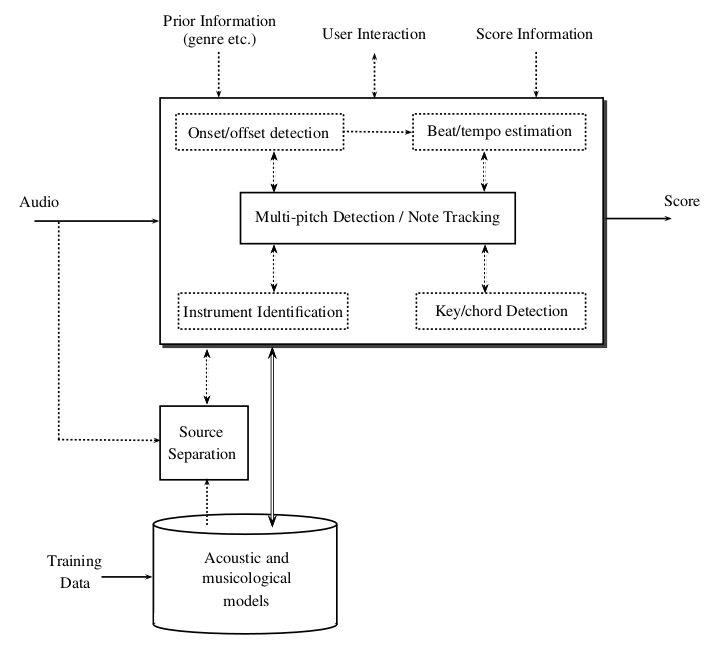
\includegraphics[height=60mm, width=60mm]{z_images/1_automatic_transcription/0_general_process.png}
	\caption{Transcription automatique}
\end{figure}
\textit{Les sous-systèmes et algorithmes optionnels sont présentés à l'aide de lignes pointillées. Les doubles flèches mettent en évidence les connexions entre les systèmes qui incluent la fusion d'informations et une communication plus interactive entre les systèmes.}\\\\
Au cœur du système se trouvent les algorithmes de détection des multi-pitchs et de suivi des notes. Quatre sous-tâches de transcription liées à la détection des hauteurs multiples et au suivi des notes apparaissent comme des algorithmes facultatifs du système (cases en pointillé) qui peuvent être intégrés dans un système de transcription. Il s'agit de l'identification de l'instrument, de l'estimation de la tonalité et de l'accord, de la détection de l'apparition et du décalage, et de l'estimation du tempo et du rythme. La séparation des sources, un problème indépendant mais lié, pourrait être traitée par un système séparé qui pourrait informer et interagir avec le système de transcription en général, et plus spécifiquement avec le sous-système d'identification des instruments.
En option, des informations peuvent également être fournies de manière externe au système de transcription. Elles peuvent être données sous forme d'informations préalables (c'est-à-dire le genre, l'instrumentation, etc.), via l'interaction de l'utilisateur ou en fournissant des informations à partir d'une partition préexistante partiellement correcte ou incomplète. Enfin, les données de formation peuvent être utilisées pour apprendre des modèles acoustiques et musicologiques qui, par la suite, informent le système de transcription et interagissent avec lui. avec le système de transcription.\\
Les applications de l’AMT ont aussi de la valeur dans les domaines oraux ou d’improvisation qui manquent de partition (jazz, pop) \cite{article1}. Les applications de l’ADT serait utile pour ces styles de musiques puisque la batterie y est amplement représentée. Un grand nombre travaux ont déjà été menés dans le domaine de l’ADT. La plupart ont été énumérés par Wu et al. \cite{8350302} qui, pour mieux comprendre la pratique des systèmes d’ADT, se concentrent sur les méthodes basées sur la factorisation matricielle non négative et celles utilisant des réseaux neuronaux récurrents.\\
La batterie a un statuts à part dans l’univers de l’AMT puisqu'il s'agit d'instruments sans hauteur, d'événements auxquels une durée est rarement attribuée et de notations spécifiques (par exemple sur les têtes de notes). Si les ordinateurs étaient capables d'analyser la partie de la batterie dans la musique enregistrée, cela permettrait une variété de tâches de traitement de la musique liées au rythme. En particulier, la détection et la classification des événements sonores de la batterie par des méthodes informatiques est considérée comme un problème de recherche important et stimulant dans le domaine plus large de la recherche d'informations musicales \cite{8350302}. Cependant, la plupart des travaux déjà entrepris se concentrent sur des méthodes de calcul pour la détection d'événements sonores de batterie à partir de signaux acoustiques ou sur la séparation entre les évènement sonore de batterie avec ceux des autres instruments dans un orchestre ou un groupe de musique \cite{2802}, ainsi que sur l'extraction de caractéristiques de bas niveau telles que la classe d'instrument et le moment de l'apparition du son. Très peu d'entre eux ont abordé la tâche de générer des partitions de batterie.

\section*{Conclusion}
Dans le cas, de l’ADT, l’architecture reste la même mais de nombreuse seront à affiner, notamment pour les questions de continuation ainsi que celle des ghost-notes et des accents.